\documentclass[letterpaper,addpoints]{exam}
\usepackage{amsmath}
\usepackage{graphicx}
\usepackage{multicol}
\usepackage{pgf}
\usepackage{tikz}
\usepackage{circuitikz}
\usetikzlibrary{arrows,shapes,trees}

\usepackage{xspace}
\newcommand{\Ohm}{$\Omega$\xspace}

\begin{document}

\begin{coverpages}
 \large\bfseries
 
 \noindent 
 Physics 252: Electronics
 
 \vspace{2ex}
 \noindent
 Final Exam: May 4, 2015

 \vspace{5ex}
 \noindent 
 Name:\enspace\makebox[2in]{\hrulefill}\\

 \vspace{5ex}
 \noindent 
 This test is administered under the rules and regulations of the honor 
 code of the College of William \& Mary.  

 \vspace{5ex}
 \noindent 
 \begin{itemize}
  \item Show your work, and \textbf{circle your answers}.
  \item You can use your notes, your lab book and the text book.
  \item The lecture slides or lab manuals are not allowed.
 \end{itemize}

 \vspace{5ex}
 \begin{center}
  \gradetable[v][questions]
 \end{center}
\end{coverpages}
 

\begin{questions}
\begin{question}[1]
How much is $1 + 1$?
\vspace{1in}
\end{question}

\begin{question}[20]
Analogous to what we did in the last stage of the full-wave rectifier circuit, an $RC$ circuit can be used to buffer an output voltage so that it never falls below a given value.  Consider a time-dependent input voltage
\begin{equation}
 v(t) =
  \begin{cases}
   V_0, & \mbox{if } 0 < t < T, 2T < t < 3T,\ldots \\
   0,   & \mbox{if } T < t < 2T, 3T < t < 4T,\ldots
  \end{cases}
\end{equation}
where the half-period $T$ is 0.1\,s and the voltage $V_0$ is 5\,V.  Design an $RC$ circuit such that the output voltage never falls below $V_0 / 2$.
\end{question}

\pagebreak

\begin{question}
For the circuits shown below specify if it is a low-pass, high-pass, band-pass or band-reject filter.

{\bf Hint:} It may be useful to think about the transfer function at high and low frequencies.
\begin{parts}
 \part[2] Circle one: band-pass \quad low-pass \quad high-pass \quad band-reject
 \begin{flushleft}
 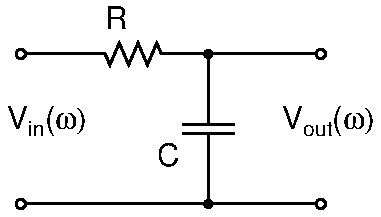
\includegraphics[height=0.7in]{./schematics/rc_low_pass}
 \end{flushleft}

 \part[2] Circle one: band-pass \quad low-pass \quad high-pass \quad band-reject
 \begin{flushleft}
 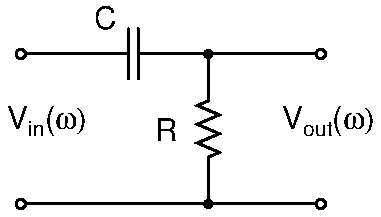
\includegraphics[height=0.7in]{./schematics/rc_high_pass}
 \end{flushleft}

 \part[2] Circle one: band-pass \quad low-pass \quad high-pass \quad band-reject
 \begin{flushleft}
 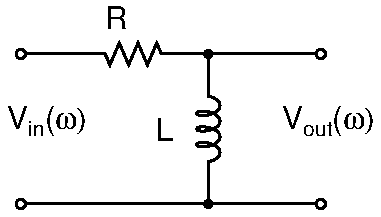
\includegraphics[height=0.7in]{./schematics/rl_high_pass}
 \end{flushleft}

 \part[2] Circle one: band-pass \quad low-pass \quad high-pass \quad band-reject
 \begin{flushleft}
 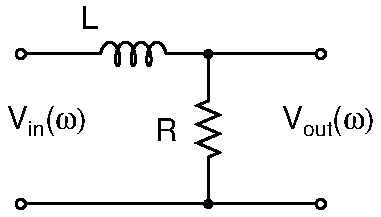
\includegraphics[height=0.7in]{./schematics/rl_low_pass}
 \end{flushleft}
 
 \part[3] Circle one: band-pass \quad low-pass \quad high-pass \quad band-reject
 \begin{flushleft}
 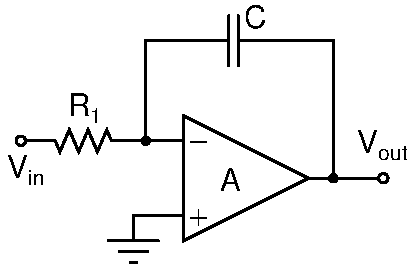
\includegraphics[height=1in]{./schematics/integrator}
 \end{flushleft}

 \part[3] Circle one: band-pass \quad low-pass \quad high-pass \quad band-reject
 \begin{flushleft}
 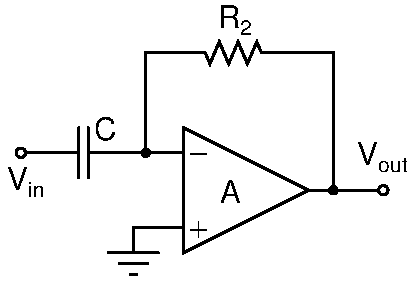
\includegraphics[height=1in]{./schematics/differentiator}
 \end{flushleft}

 \part[5] Circle one: band-pass \quad low-pass \quad high-pass \quad band-reject
 \begin{flushleft}
 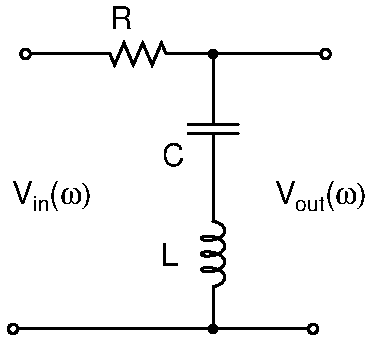
\includegraphics[height=1.1in]{./schematics/rlcnotch}
 \end{flushleft}

 \pagebreak

 \part[5] Circle one: band-pass \quad low-pass \quad high-pass \quad band-reject
 \begin{flushleft}
 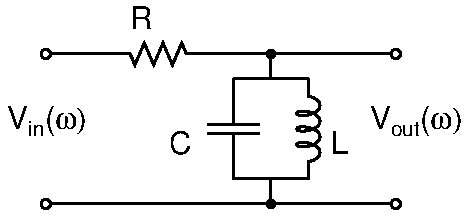
\includegraphics[height=0.7in]{./schematics/rlc_band_pass}
 \end{flushleft}

 \part[5] Circle one: band-pass \quad low-pass \quad high-pass \quad band-reject
 \begin{flushleft}
 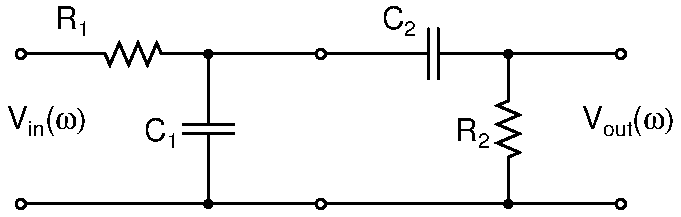
\includegraphics[height=0.7in]{./schematics/band_pass_filter}
 \end{flushleft}
\end{parts}
\end{question}

\pagebreak

\begin{question}[10]
You are hired as a research assistant for an electronics lab. Your first assignment is to characterize a black box (which seems to be a power supply) given to you.

In a nearby lab book you find a series of measurements on this box. In particular you find the voltage drop across several load resistors connected to the box (see the table below).

\begin{center}
 \begin{tabular}{|c|c|}
  \hline
   $R_L$         &  $V_L$ \\ 
  \hline
   1\,k$\Omega$  &  10\,V \\
   100\,$\Omega$ &  2\,V  \\
  \hline
 \end{tabular}
\end{center}
 
Find the equivalent Th\'{e}venin voltage and Th\'{e}venin resistance of this black box. 
\begin{solution}[2in]
The Th\'evenin voltage is $V_{Th} = V_L + R_{Th} I_L = V_L + R_{Th} V_L / R_L$.  This gives us two equations, which we can subtract to find $0 = (10\,\hbox{V} - 2\,\hbox{V}) + R_{Th} (10\,\hbox{mA} - 20\,\hbox{mA})$.  We solve for $R_{Th}$ and find $R_{Th} = 800\,\Omega$, and then $V_{Th} = 18\,\hbox{V}$.
\end{solution}
\end{question}

\pagebreak

\begin{question}
Consider the inverting amplifier in Figure~\ref{fig:inverting_amplifier}.  
\begin{figure}
\begin{center}
\begin{circuitikz}
\draw (0,0) node[op amp](opamp){$A$};
\draw (opamp.-) to[R,l=$R_1$,-o] ++(-2,0) node[left]{$v_{in}$};
\draw (opamp.+) to[short] ++(-0.5,0) node[ground]{};
\draw (opamp.out) to[short,-o] ++(0.5,0) node[right]{$v_{out}$};
\draw (opamp.out) to[short] ++(0,1.5) to[R,l=$R_2$] ++(-2,0) -| (opamp.-);
\end{circuitikz}
\end{center}
\caption{Inverting amplifier.}
\label{fig:inverting_amplifier}
\end{figure}

\begin{parts}
\part[10] Find the expression for the output voltage $v_{out}$ in terms of $v_{in}$, $R_1$, $R_2$, and $A$. Do not assume that the op amp open-loop gain $A$ is infinite.
\vspace{4in}
\part[5] If the gain-bandwidth product of the op amp is $A(f) \cdot f = 10$\,MHz, with $R_2/R_1 = 10$, what will the gain $G(f)$ be at $f = 10$\,Hz and at $f = 10$\,MHz?
\vspace{3in}
\part[5] Assume now that $A \to \infty$, $R_2/R_1 = 10$ and $v_{in} = 100$\,mV, but that the maximum possible output current of the op amp is 20\,mA.  What is the minimum possible load resistor that you can connect to the output without overloading the op amp?
\vspace{3in}
\end{parts}
\end{question}

\pagebreak

\begin{question}
Consider the relaxation oscillator with an open collector comparator in Figure~\ref{fig:relaxation_oscillator}.
\begin{figure}
\begin{center}
\begin{circuitikz}
\draw (0,0) node[op amp, yscale=-1](opamp){};
\draw (opamp.-) to[short] ++(0,-1) node[circ](fb){} to[R,l=$R$] ++(2,0) -| (opamp.out);
\draw (fb) to[C,l_=$C$] ++(-1,0) node[ground]{};
\draw (opamp.out) node[circ]{} to[short] ++(0.5,0)  node[circ](out){} to[short,-o] ++(0.5,0) node[right]{$V_{out}$};
\draw (opamp.+) node[circ](in1){} to[short] ++(0,+1.5) to[R,l=100\,k\Ohm] ++(2,0) -| (opamp.out);
\draw (out) to[R,l_=$R_{pull-up}$,-o] ++(0,2.5) node[above]{5\,V};
\draw (in1) to[short] ++(-1.75,0) node[circ](in2){} to[R,l=100\,k\Ohm,-o] ++(0,2) node[above]{5\,V};
\draw (in2) to[R,l_=100\,k\Ohm] ++(0,-2.0) node[ground]{};
\end{circuitikz}
\end{center}
\caption{A square wave generator made using a relaxation oscillator.}
\label{fig:relaxation_oscillator}
\end{figure}
\begin{parts}
\part[4] Disregarding the effects of $R_{pull-up}$, what is the voltage at the non-inverting input when the output is high?
\vspace{2in}
\part[4] Disregarding the effects of $R_{pull-up}$, what is the voltage at the non-inverting input when the output is low?
\vspace{2in}
\part[6] If the resistor $R$ has a value of 1\,M\Ohm, what should the value for the capacitor $C$ be to obtain a period of 1\,ms?
\vspace{2in}
\part[6] When we used a relaxation oscillator to blink an LED, we found that connecting the LED directly between the output and ground did not work as expected due to the large output impedance.  What is the output impedance of the relaxation oscillator?
\vspace{2in}
\end{parts}
\end{question}

\end{questions}

\end{document}
